\chapter{Experimental Setup and Results Analysis}
\label{ch:results}

\section{Experimental Setup}
\label{sec:env}
All experiments ran on one laptop with an AMD Ryzen 7 6800H CPU (8 cores),
15.3 GB of memory and no GPU, under Windows 11 with Python 3.10.11, PyTorch
2.14.1, PennyLane 0.42.3, scikit-learn~\cite{pedregosa2011} 1.7.2 and NumPy
2.2.6. Circuits were simulated exactly with \texttt{default.qubit}, except
in the noise experiments, which used finite shots and the
\texttt{default.mixed} density-matrix simulator. Each experiment is a
separate script that writes its configuration and metrics to
\texttt{results/tb/}. Because the laptop was shared, training times varied
between runs and are given as rough indications only. All results refer to
the same 630 test images (525 normal, 105 TB).

In a first single-seed run (seed 42), replacing the 33-parameter linear head
with the 161-parameter quantum head raised accuracy from 97.46\% to 98.41\%
(16 errors against 10; missed TB cases 9 against 7) at about three times the
training time. Since the two models differ in more than the circuit, the
following experiments use repeated seeds and matched controls.

\section{Circuit Design Ablation}
\label{sec:res_ablation}
The ablation varies one property of the \cq{} circuit at a time, starting
from 4 qubits, depth 2, angle encoding and strong entanglement (seed 42).
Figure~\ref{fig:ablation} shows all twelve configurations on a common axis.

\begin{figure}[htbp]
  \centering
  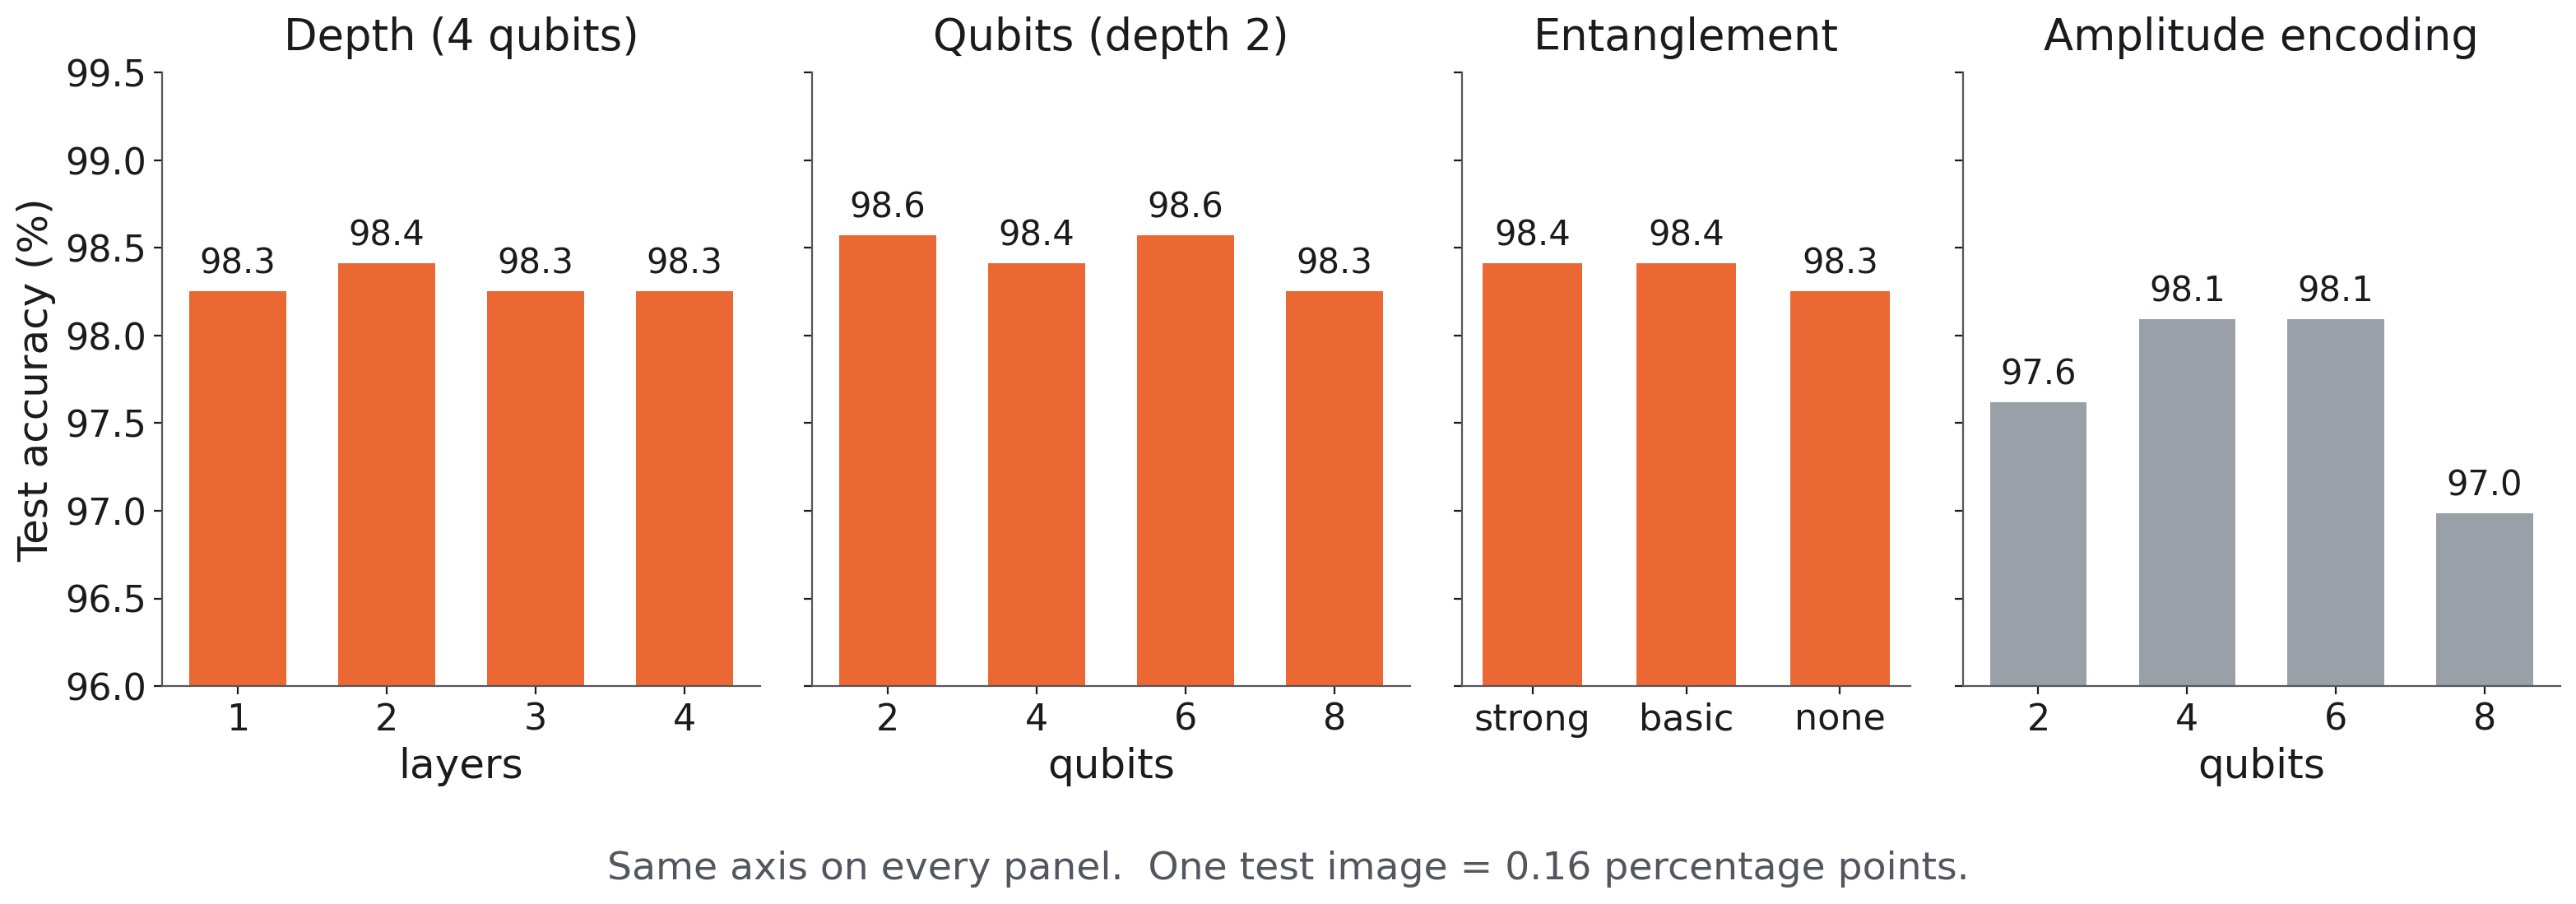
\includegraphics[width=\linewidth]{ablation_summary.png}
  \caption{Test accuracy of all twelve circuit configurations of the \cq{}
  hybrid (seed 42). All panels share one axis; one test image corresponds to
  0.16 percentage points.}
  \label{fig:ablation}
\end{figure}

Depth changed test accuracy only between 98.25\% and 98.41\%, one test
image, while training time grew roughly linearly with depth; the best
validation F1 was obtained at depth 1. Strong and basic entanglement gave
identical results (98.41\%, F1 0.9515), and removing entanglement cost a
single test image. With angle encoding, 2 to 8 qubits gave 98.25--98.57\%.
Amplitude encoding was worse in every case (96.98--98.10\%) and worst at 8
qubits, where 256 amplitudes must be produced from a 32-dimensional
embedding and normalisation discards the vector's length. Within the tested
range the circuit design therefore barely affects accuracy: after the CNN
has extracted its features, the four-to-one decision does not need the
extra correlations that entanglement provides. Angle encoding is
consistently preferable, and small circuits are as good as large ones.

\section{Backbone and Head Comparison}
\label{sec:res_backbone}
The third experiment crosses two backbones with two heads, each with three
seeds (Table~\ref{tab:comparison}).

\begin{table}[htbp]
\centering
\footnotesize
\caption{Backbone $\times$ head comparison: mean $\pm$ standard deviation over seeds 42, 43 and 44 on the fixed test set.}
\label{tab:comparison}
\begin{adjustbox}{max width=\linewidth}
\begin{tabular}{lrrrrrrr}
\toprule
Model & Params & Accuracy (\%) & Precision & Recall & F1 & ROC-AUC & Time (s) \\
\midrule
CNN + classical & 132,385 & 98.04 $\pm$ 0.56 & 0.9326 $\pm$ 0.0286 & 0.9524 $\pm$ 0.0381 & 0.9418 $\pm$ 0.0172 & 0.9975 $\pm$ 0.0004 & 16 \\
CNN + quantum & 132,513 & 98.41 $\pm$ 0.32 & 0.9612 $\pm$ 0.0094 & 0.9429 $\pm$ 0.0165 & 0.9519 $\pm$ 0.0098 & 0.9980 $\pm$ 0.0014 & 46 \\
ResNet18 + classical & 11,192,961 & 99.21 $\pm$ 0.57 & 0.9875 $\pm$ 0.0216 & 0.9651 $\pm$ 0.0361 & 0.9758 $\pm$ 0.0178 & 0.9991 $\pm$ 0.0006 & 314 \\
ResNet18 + quantum & 11,193,089 & 99.47 $\pm$ 0.18 & 0.9936 $\pm$ 0.0056 & 0.9746 $\pm$ 0.0145 & 0.9839 $\pm$ 0.0057 & 0.9961 $\pm$ 0.0046 & 346 \\
\bottomrule
\end{tabular}
\end{adjustbox}
\end{table}


With both backbones the quantum head gave a higher mean accuracy and F1 and
a smaller standard deviation: $98.41 \pm 0.32\%$ against $98.04 \pm 0.56\%$
for the small CNN, and $99.47 \pm 0.18\%$ against $99.21 \pm 0.57\%$ for
ResNet18. The backbone mattered about three times more than the head:
ResNet18 raised accuracy by about one percentage point, at the cost of 85
times more parameters and about 20 times longer training. ROC-AUC exceeded
0.996 for every model, so all four rank images almost perfectly and the
differences lie in where the 0.5 threshold falls. The head differences are
comparable to the seed-to-seed variation and are tested for significance
next.

\section{Main Study: Hybrids versus Matched Controls}
\label{sec:res_study}
The main experiment trains the seven models of Table~\ref{tab:controls}
with three seeds on five training-set sizes (105 runs).
Table~\ref{tab:study_full} gives the full-data results and
Table~\ref{tab:mcnemar} the paired tests.

\begin{table}[htbp]
\centering
\footnotesize
\caption{Main study on the full training set (2,940 images): mean $\pm$ std over three seeds. Head parameters count only the classifier head.}
\label{tab:study_full}
\begin{adjustbox}{max width=\linewidth}
\begin{tabular}{lrrrrrrr}
\toprule
Model & Params & Head & Accuracy (\%) & Recall & F1 & ROC-AUC & Time (s) \\
\midrule
Classical CNN & 132,385 & 33 & 97.67 $\pm$ 0.33 & 0.9238 $\pm$ 0.0095 & 0.9298 $\pm$ 0.0094 & 0.9966 $\pm$ 0.0009 & 15 \\
CNN + matched classical head & 132,509 & 157 & 97.72 $\pm$ 0.40 & 0.9079 $\pm$ 0.0145 & 0.9301 $\pm$ 0.0119 & 0.9959 $\pm$ 0.0011 & 17 \\
C$\rightarrow$Q hybrid (CNN + quantum head) & 132,513 & 161 & 98.41 $\pm$ 0.32 & 0.9429 $\pm$ 0.0165 & 0.9519 $\pm$ 0.0098 & 0.9980 $\pm$ 0.0014 & 43 \\
Q$\rightarrow$C hybrid (quanvolution + CNN) & 34,297 & 33 & 97.88 $\pm$ 0.33 & 0.9270 $\pm$ 0.0145 & 0.9359 $\pm$ 0.0096 & 0.9954 $\pm$ 0.0017 & 5 \\
Random patch + CNN (control) & 34,297 & 33 & 90.53 $\pm$ 0.87 & 0.5206 $\pm$ 0.0715 & 0.6449 $\pm$ 0.0543 & 0.9336 $\pm$ 0.0035 & 4 \\
Avg-pool + CNN (control) & 34,081 & 33 & 98.15 $\pm$ 0.09 & 0.9556 $\pm$ 0.0110 & 0.9451 $\pm$ 0.0020 & 0.9956 $\pm$ 0.0008 & 4 \\
Learned 2x2 conv + CNN (control) & 34,317 & 33 & 98.31 $\pm$ 0.72 & 0.9524 $\pm$ 0.0000 & 0.9497 $\pm$ 0.0204 & 0.9956 $\pm$ 0.0033 & 7 \\
\bottomrule
\end{tabular}
\end{adjustbox}
\end{table}

\begin{table}[htbp]
\centering
\scriptsize
\caption{McNemar exact test between each hybrid and a classical comparator on the full-data runs. Each cell gives the p-value and, in brackets, the number of test images only the hybrid got right / only the comparator got right.}
\label{tab:mcnemar}
\begin{adjustbox}{max width=\linewidth}
\begin{tabular}{llrrr}
\toprule
Hybrid & Compared with & Seed 42 & Seed 43 & Seed 44 \\
\midrule
C$\rightarrow$Q hybrid (CNN + quantum head) & CNN + matched classical head & 0.092 (10/3) & 0.146 (9/3) & 1.000 (7/7) \\
Q$\rightarrow$C hybrid (quanvolution + CNN) & Random patch + CNN (control) & $<$0.001 (57/2) & $<$0.001 (49/7) & $<$0.001 (50/8) \\
Q$\rightarrow$C hybrid (quanvolution + CNN) & Avg-pool + CNN (control) & 1.000 (5/4) & 0.344 (3/7) & 0.791 (6/8) \\
Q$\rightarrow$C hybrid (quanvolution + CNN) & Learned 2x2 conv + CNN (control) & 1.000 (4/4) & 1.000 (6/6) & 0.057 (3/11) \\
C$\rightarrow$Q hybrid (CNN + quantum head) & Classical CNN & 0.424 (9/5) & 0.227 (8/3) & 0.267 (9/4) \\
Q$\rightarrow$C hybrid (quanvolution + CNN) & Classical CNN & 0.453 (5/2) & 0.804 (7/9) & 0.581 (8/5) \\
\bottomrule
\end{tabular}
\end{adjustbox}
\end{table}


\paragraph{Does the quantum head help?} The \cq{} hybrid was the best
small-CNN model ($98.41 \pm 0.32\%$, F1 $0.952 \pm 0.010$). Its matched
classical control, with the same bottleneck, scored $97.72 \pm 0.40\%$ and
$0.930 \pm 0.012$, almost exactly like the plain CNN ($97.67 \pm 0.33\%$,
$0.930 \pm 0.009$), so the bottleneck alone does not explain the gain, and
the hybrid was ahead for every seed. The McNemar tests, however, are not
significant: $p$ = 0.092, 0.146 and 1.000 against the matched head and
0.424, 0.227 and 0.267 against the CNN. With error rates around 2\%, two
models disagree on only a handful of the 630 images, too few to rule out
chance. The quantum head thus gives a small, consistent improvement of
about 0.7 percentage points that this dataset cannot confirm statistically.

\paragraph{Does the quantum filter help?} The \qc{} hybrid reached
$97.88 \pm 0.33\%$ with 34,297 parameters, indistinguishable from the
132,385-parameter CNN ($p$ = 0.453, 0.804, 0.581). It was far better than
the random classical patch map ($90.53\%$, $p < 0.001$ for every seed),
whose $\tanh$ saturates and turns patches into nearly binary values, while
the quantum filter's cosine-shaped response keeps the detail. But
$2\times2$ average pooling ($98.15 \pm 0.09\%$) and a learned $2\times2$
convolution ($98.31 \pm 0.72\%$) did as well as the quantum filter
($p \geq 0.057$). The four-fold parameter saving therefore comes from
halving the resolution, not from the quantum computation, mirroring the
finding of Henderson et al.~\cite{henderson2020}.

\paragraph{Low-data regime.} Table~\ref{tab:study_lowdata} gives F1 for
smaller training sets. With 2\% of the data (58 images), the \qc{} hybrid
and average pooling had the highest F1 (0.677 and 0.666), and the \qc{}
hybrid was by far the most stable model (standard deviation 0.020). The
four-dimensional bottleneck heads were unreliable with little data: the
matched classical head predicted ``Normal'' for every test image in all
three seeds at 2\% and in two of three seeds at 5\% and 25\%, and the \cq{}
hybrid reached only $0.341 \pm 0.250$ at 2\%. This is a calibration failure
rather than a failure to learn: at 2\% the \cq{} hybrid had the
\emph{highest} ROC-AUC of all models (0.927 against 0.911 for the CNN), so it
ranks images well but its probabilities do not cross the 0.5 threshold in
the right places. From 5\% upwards the classical CNN had the highest or
joint-highest F1, and only with the full data did the \cq{} hybrid move
ahead. The experiment therefore does not support a general claim that the
hybrids learn more from fewer examples.

\begin{table}[htbp]
\centering
\scriptsize
\caption{Test F1 (mean $\pm$ std, three seeds) versus the fraction of the training split used. Validation and test sets are never reduced.}
\label{tab:study_lowdata}
\begin{adjustbox}{max width=\linewidth}
\begin{tabular}{lrrrrr}
\toprule
Model & 2\% (58) & 5\% (147) & 10\% (294) & 25\% (735) & 100\% (2940) \\
\midrule
Classical CNN & 0.601 $\pm$ 0.170 & 0.815 $\pm$ 0.027 & 0.880 $\pm$ 0.009 & 0.909 $\pm$ 0.008 & 0.930 $\pm$ 0.009 \\
CNN + matched classical head & 0.000 $\pm$ 0.000 & 0.263 $\pm$ 0.455 & 0.876 $\pm$ 0.010 & 0.309 $\pm$ 0.535 & 0.930 $\pm$ 0.012 \\
C$\rightarrow$Q hybrid (CNN + quantum head) & 0.341 $\pm$ 0.250 & 0.787 $\pm$ 0.064 & 0.850 $\pm$ 0.077 & 0.871 $\pm$ 0.080 & 0.952 $\pm$ 0.010 \\
Q$\rightarrow$C hybrid (quanvolution + CNN) & 0.677 $\pm$ 0.020 & 0.754 $\pm$ 0.093 & 0.834 $\pm$ 0.028 & 0.884 $\pm$ 0.015 & 0.936 $\pm$ 0.010 \\
Random patch + CNN (control) & 0.000 $\pm$ 0.000 & 0.416 $\pm$ 0.086 & 0.456 $\pm$ 0.065 & 0.490 $\pm$ 0.052 & 0.645 $\pm$ 0.054 \\
Avg-pool + CNN (control) & 0.666 $\pm$ 0.138 & 0.749 $\pm$ 0.099 & 0.862 $\pm$ 0.020 & 0.892 $\pm$ 0.011 & 0.945 $\pm$ 0.002 \\
Learned 2x2 conv + CNN (control) & 0.451 $\pm$ 0.076 & 0.705 $\pm$ 0.155 & 0.768 $\pm$ 0.092 & 0.857 $\pm$ 0.075 & 0.950 $\pm$ 0.020 \\
\bottomrule
\end{tabular}
\end{adjustbox}
\end{table}


\section{Quantum Circuit Analysis}
\label{sec:res_expr}
Figure~\ref{fig:expr} characterises the trainable block of the \cq{}
circuit without any data. With entangling gates, expressibility improves
sharply from depth 1 to depth 2 (KL divergence 0.308 to 0.0083 for strong
entanglement) and reaches 0.004--0.005 at depth 3, close to Haar-random.
Without entanglement it stays at 0.19--0.30 whatever the depth, because
product states can never cover the four-qubit state space. The entangling
capability of the strong and basic patterns is 0.79--0.87, close to the
Haar-random value $14/17 \approx 0.82$, and exactly zero without
entanglement. Read together with the ablation, the circuits differ strongly
as quantum objects --- at depths 2 to 4 the no-entanglement circuit is 20 to
60 times less expressive --- yet give almost the same accuracy: the task, as
posed after a classical feature extractor, does not use the extra capacity.

\begin{figure}[htbp]
  \centering
  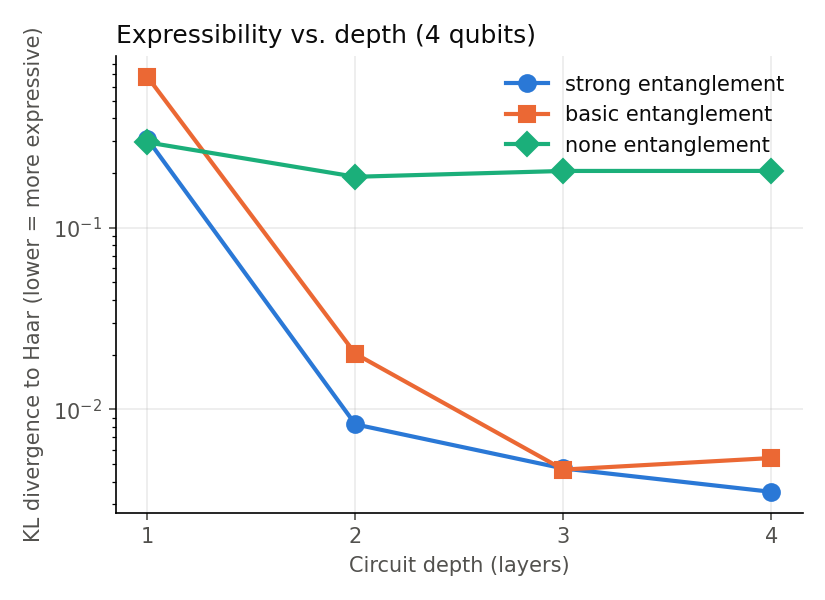
\includegraphics[width=0.48\linewidth]{expressibility.png}\hfill
  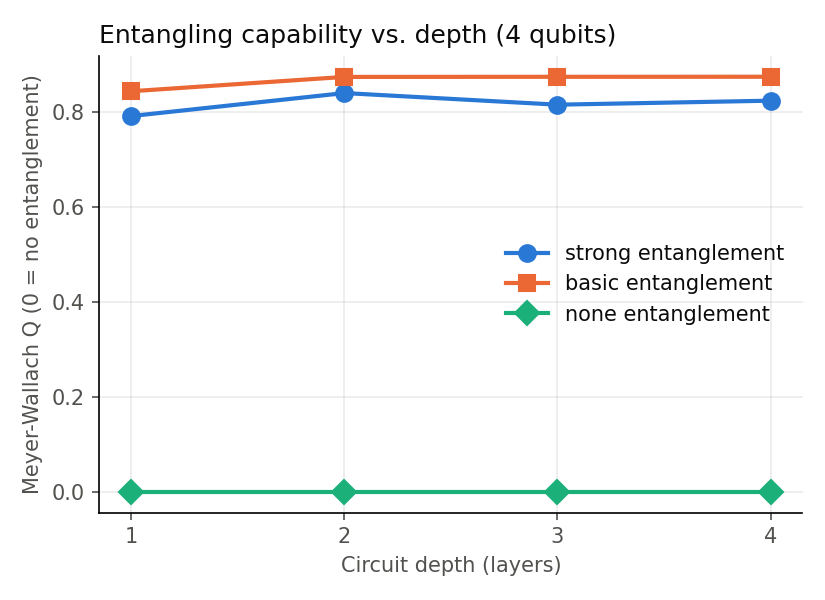
\includegraphics[width=0.48\linewidth]{entangling_capability.png}
  \caption{Expressibility (left, lower is more expressive) and entangling
  capability (right) of the three entanglement patterns versus depth,
  4 qubits.}
  \label{fig:expr}
\end{figure}

\label{sec:res_bp}
Figure~\ref{fig:bp} shows how the gradient variance scales with the number
of qubits. For depth 10 it falls from 0.150 at 2 qubits to
$4.2 \times 10^{-4}$ at 10 qubits for the local cost, and from 0.122 to
$5.0 \times 10^{-4}$ for the global cost --- about a factor of two per added
qubit, the $2^{-n}$ decay predicted by McClean et al.~\cite{mcclean2018}. The
depth-2 curves follow the same trend but are noisier, and we did not observe
the advantage of local over global costs reported by Cerezo et
al.~\cite{cerezo2021}, possibly because the long-range CNOTs spread
information across all qubits even at depth 2. At 4 qubits the variance is
60 to 300 times larger than at 10, which supports the choice of a small
circuit, particularly for hardware, where each gradient must be estimated
from finite shots.

\begin{figure}[htbp]
  \centering
  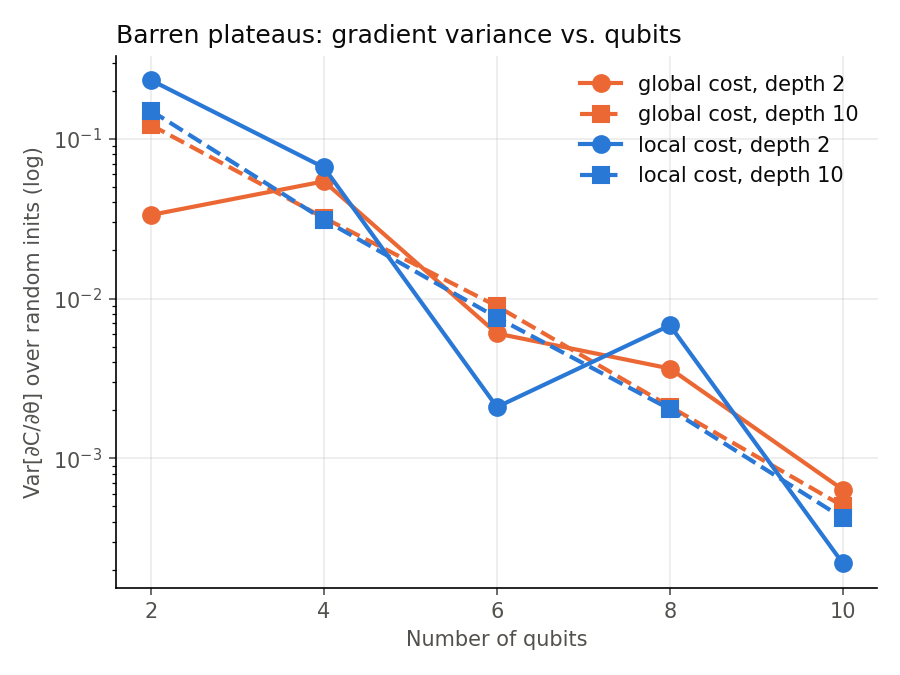
\includegraphics[width=0.6\linewidth]{barren_plateaus.png}
  \caption{Variance of the cost gradient over 500 random initialisations
  versus number of qubits for local and global costs at depths 2 and 10.}
  \label{fig:bp}
\end{figure}

\section{Robustness to Shot Noise and Hardware Noise}
\label{sec:res_noise}
Figure~\ref{fig:noise} shows the trained \cq{} model (seed 42) evaluated as
on an imperfect device. With only 10 shots per expectation value, which gives
each $\expval{Z_k}$ a standard error of up to 0.32, accuracy was 98.25\%
against 98.41\% for exact values, and with 50 to 10,000 shots it stayed
within 98.25--98.57\%. With depolarising noise after every layer it stayed
within 98.41--98.57\% up to $p = 0.2$, and the AUC was unchanged at 0.9987.
Most test images lie far from the decision boundary, and depolarisation
shrinks all four outputs by a similar factor (about 0.65--0.75 at $p = 0.1$),
so the direction of the output vector and the ranking of images are
preserved. Finally, parameter-shift and backpropagation gradients of the
trained circuit agreed to $1.1 \times 10^{-15}$, so the model could be
trained on hardware without any change. These results apply to small,
shallow circuits; deeper circuits or less uniform noise would degrade more.

\begin{figure}[htbp]
  \centering
  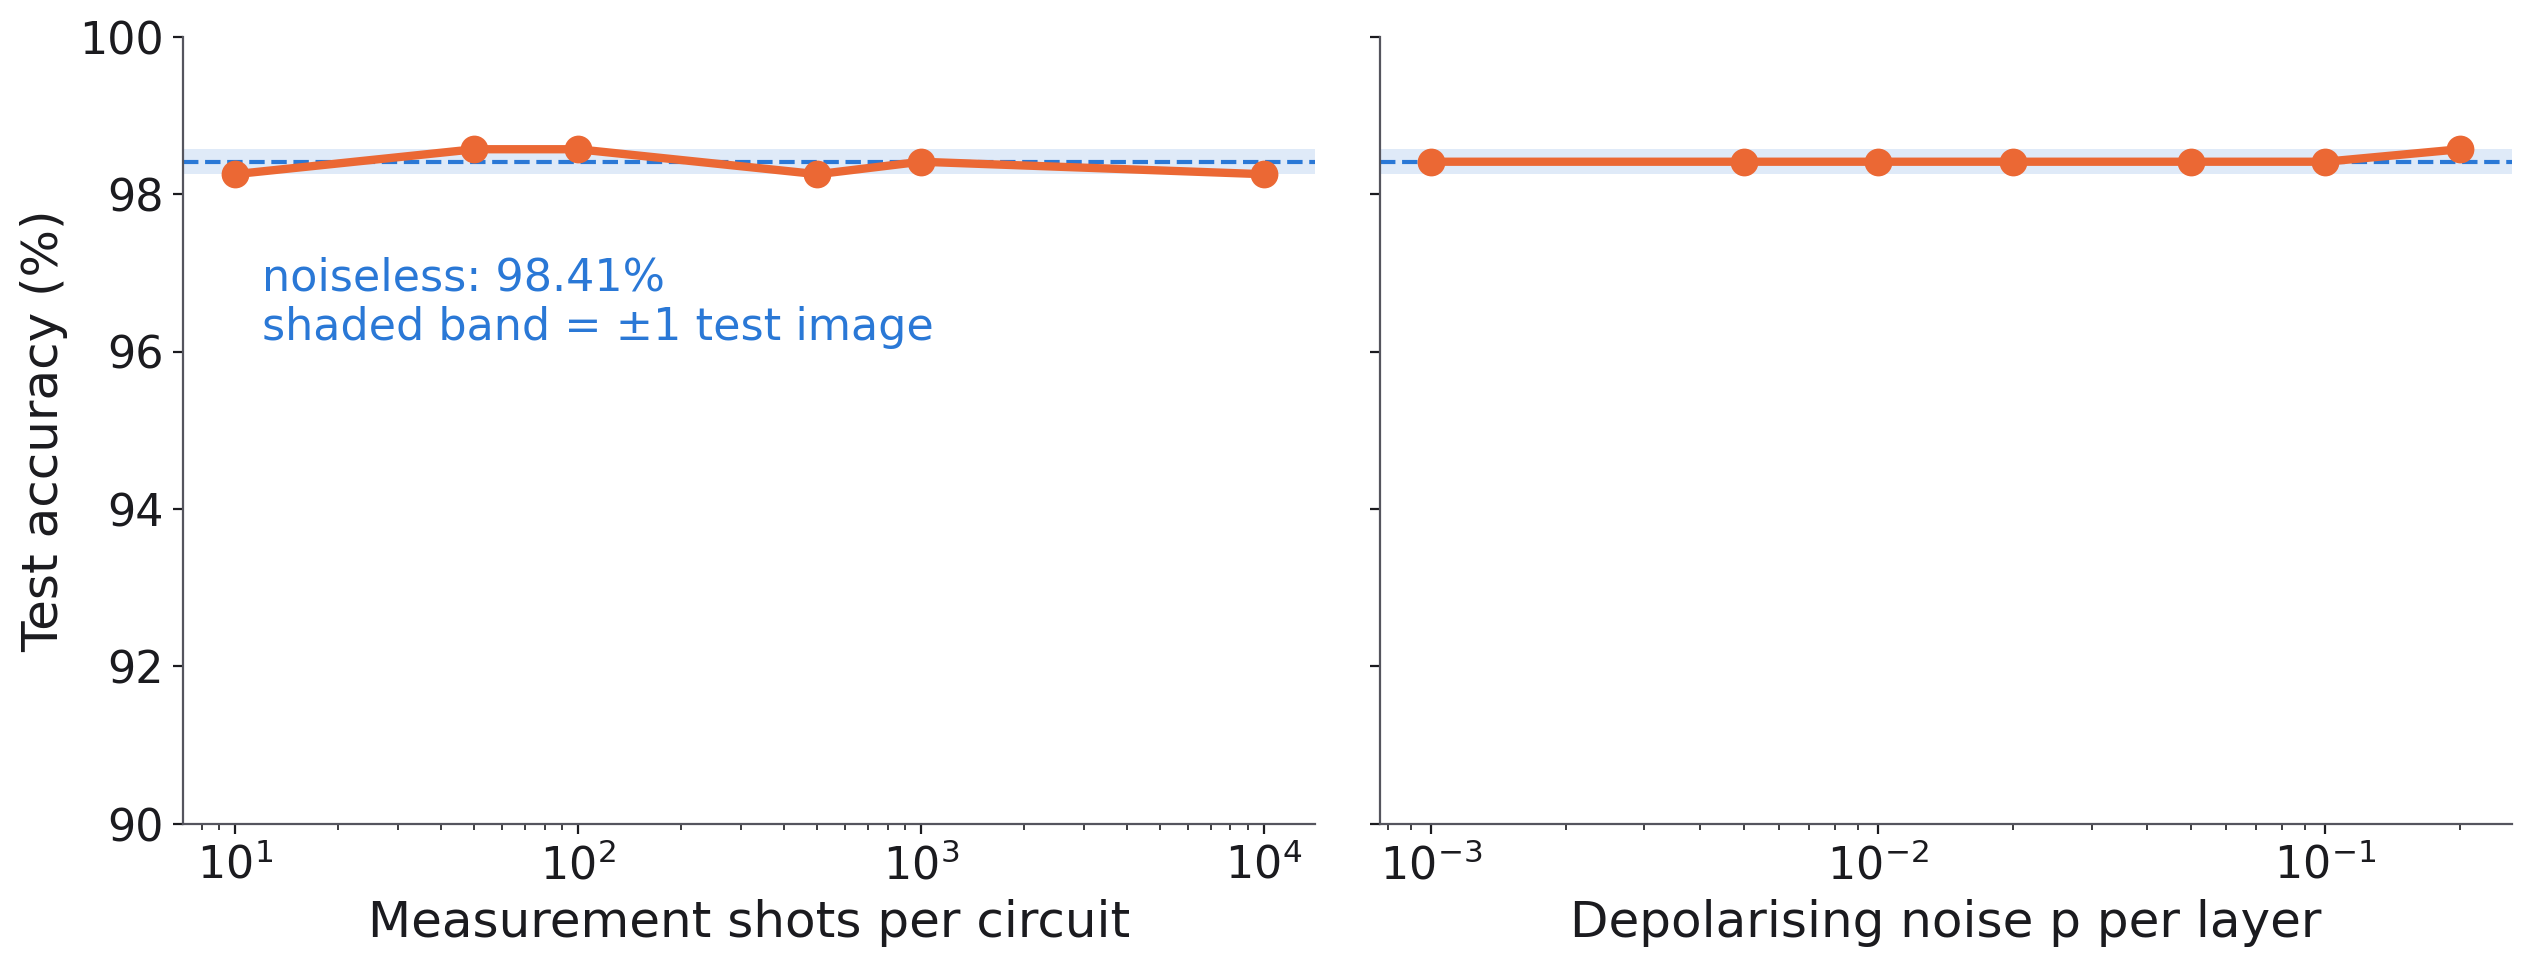
\includegraphics[width=\linewidth]{nisq_robustness.png}
  \caption{Test accuracy of the trained \cq{} model versus measurement shots
  (left) and depolarising probability per layer (right). The shaded band is
  $\pm 1$ test image around the noiseless accuracy.}
  \label{fig:noise}
\end{figure}

\section{Error Analysis}
\label{sec:res_errors}
For seed 42, only 22 of the 630 test images were misclassified by any of the
four backbone $\times$ head models, and a single image by all four. The
small-CNN models' errors were dominated by missed TB cases (9 of 16 for the
classical head, 7 of 10 for the quantum head), the more harmful error in
screening, while ResNet18 reduced the errors to one or two.
Figure~\ref{fig:errors} shows the most confident mistakes of the CNN with a
quantum head. They include TB cases with subtle changes that are hard to see
at $64 \times 64$ pixels and a normal portable film with text markers, a
reminder that models may partly learn differences between image sources
rather than disease.

\begin{figure}[htbp]
  \centering
  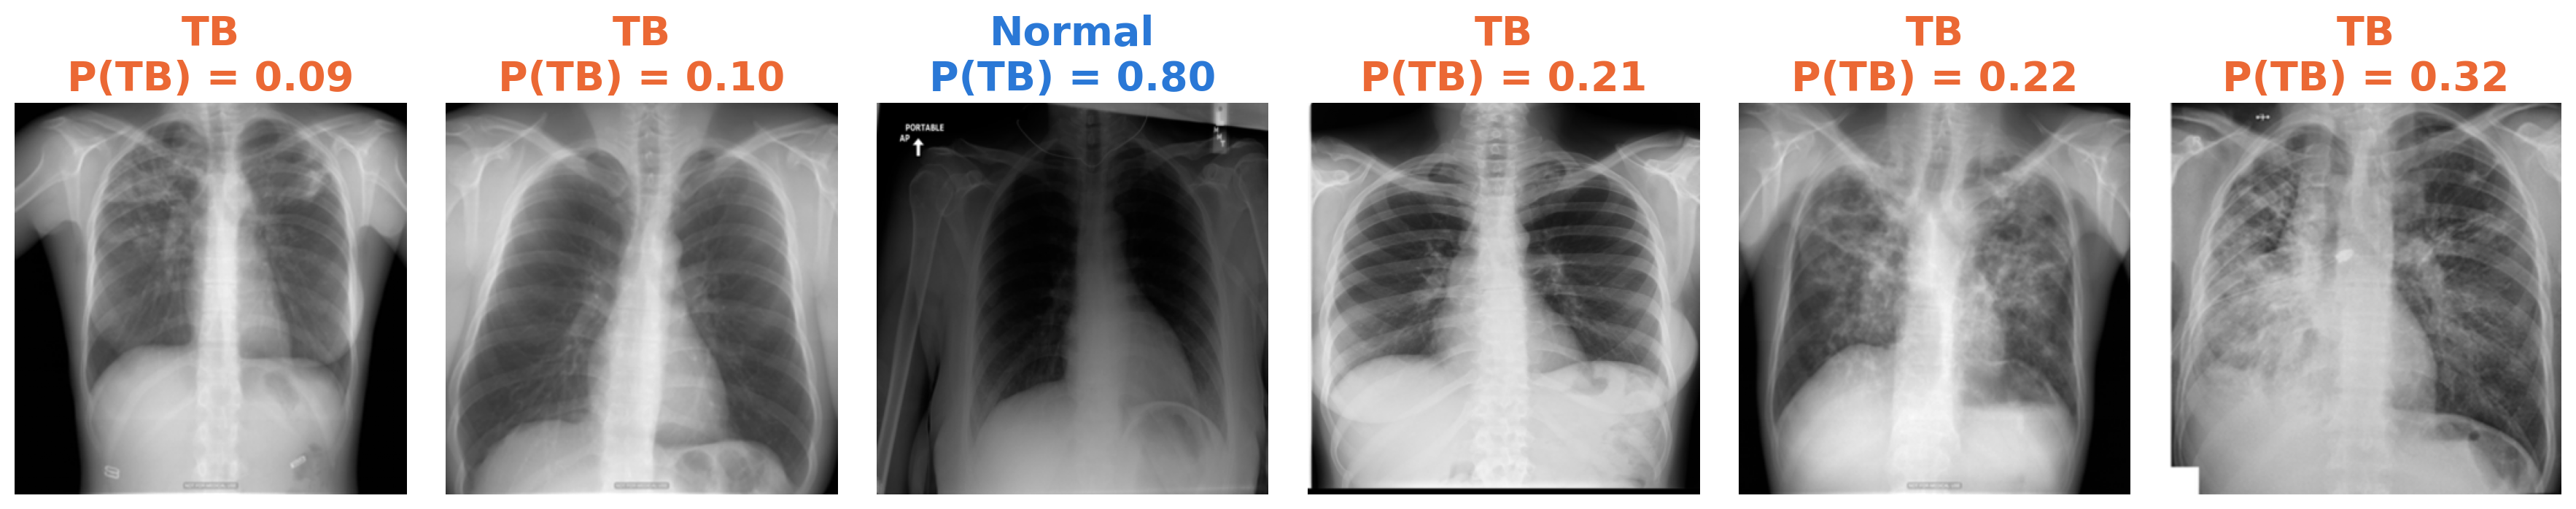
\includegraphics[width=\linewidth]{errors_labeled.png}
  \caption{The six most confident mistakes of the CNN + quantum head model
  (seed 42), with the true class and the predicted probability of TB.}
  \label{fig:errors}
\end{figure}

\section{Discussion}
\label{sec:discussion}
Rahman et al.~\cite{rahman2020} reported 98--99\% accuracy on the same
dataset with large pretrained CNNs on much larger images. Our classical CNN
(97.67\%), \cq{} hybrid (98.41\%) and ResNet18 with a quantum head
(99.47\%) fall in the same range, but the comparison is only indicative,
since splits, preprocessing and resolution differ and a 630-image test set
gives each accuracy an uncertainty of about $\pm 1$ percentage point.

Taken together, the experiments show that a quantum classifier head is a
viable drop-in replacement for a classical one, with a small, consistent but
not significant gain; that the quanvolution filter is a reasonable but not a
special feature extractor, whose efficiency comes from downsampling; that
circuit design changes expressibility by more than an order of magnitude but
accuracy by at most a test image or two; and that small hybrid circuits are
trainable and robust to the noise of current hardware. What the evidence
does \emph{not} show is a quantum advantage: no hybrid was significantly
better than its best classical counterpart, consistent with the expectation
that small, classically simulable circuits cannot outperform classical
models of similar size.
